%\documentclass[tikz]{standalone}
\documentclass[]{article}
\usepackage{pgfplots}
\usepackage{tikz}
\usepackage{graphicx}
\usetikzlibrary{arrows,positioning}
\def\subdivisions{50}
\def\blendfrac{0.5}
\tikzset{>=latex}
\def\deltaang{-155}
\def\fromang{180}
\def\inputang{-40}
\def\protrude{7}
\def\arcwidth{0.3cm}
\def\highlightrad{0.2cm}
\def\autocatalrad{1.5cm}
\def\autocatalscale{1.5}
\newcommand{\shadedarc}[7][\arcwidth]{%width,startang,stopang,startrad,stoprad,startcol,stopcol
  \foreach \i[evaluate={\col=(\i+0.5)/\subdivisions*100}] in {0,...,\numexpr\subdivisions-1\relax}
  \draw[color={#6!\col!#7},line width=#1] 
    (\i*#3/\subdivisions-\i*#2/\subdivisions+#2:#4+#5*\i/\subdivisions-#4*\i/\subdivisions)
arc[start angle=\i*#3/\subdivisions-\i*#2/\subdivisions+#2,
end angle=(\i+1.1)*#3/\subdivisions-(\i+1.1)*#2/\subdivisions+#2,radius=#4+#5*\i/\subdivisions-#4*\i/\subdivisions];

}
\newcommand{\coloredarc}[6][\arcwidth]{%width,startang,stopang,startrad,stoprad,startcol,stopcol
  \foreach \i in {0,...,\numexpr\subdivisions-1\relax}
  \draw[color={#6},line width=#1] 
    (\i*#3/\subdivisions-\i*#2/\subdivisions+#2:#4+#5*\i/\subdivisions-#4*\i/\subdivisions)
arc[start angle=\i*#3/\subdivisions-\i*#2/\subdivisions+#2,
end angle=(\i+1.1)*#3/\subdivisions-(\i+1.1)*#2/\subdivisions+#2,radius=#4+#5*\i/\subdivisions-#4*\i/\subdivisions];

}
%cbbcolors
\colorlet{cbbinit}{green}
\definecolor{cbbmed}{rgb}{1,1,-1}
\definecolor{cbbext}{rgb}{-0.5,-0.5,1}
%glycolors
\colorlet{glyinit}{magenta}
\definecolor{glymed}{rgb}{-0.5,-0.5,1}
\definecolor{glyext}{rgb}{1,-0.5,-0.5}
\colorlet{glyinter}{glymed!50!glyext}
%ptscolors
\colorlet{ptsinit}{cyan}
\definecolor{ptsmed}{rgb}{-0.5,-0.5,1}
\colorlet{ptsext}{green}
\colorlet{gluccol}{green!50!black}
%gencolors
\colorlet{genmed}{red}
\colorlet{genext}{green}
\colorlet{geninit}{red!50!green}
\begin{document}

\begin{figure}
    \resizebox{1.3\linewidth}{!}{
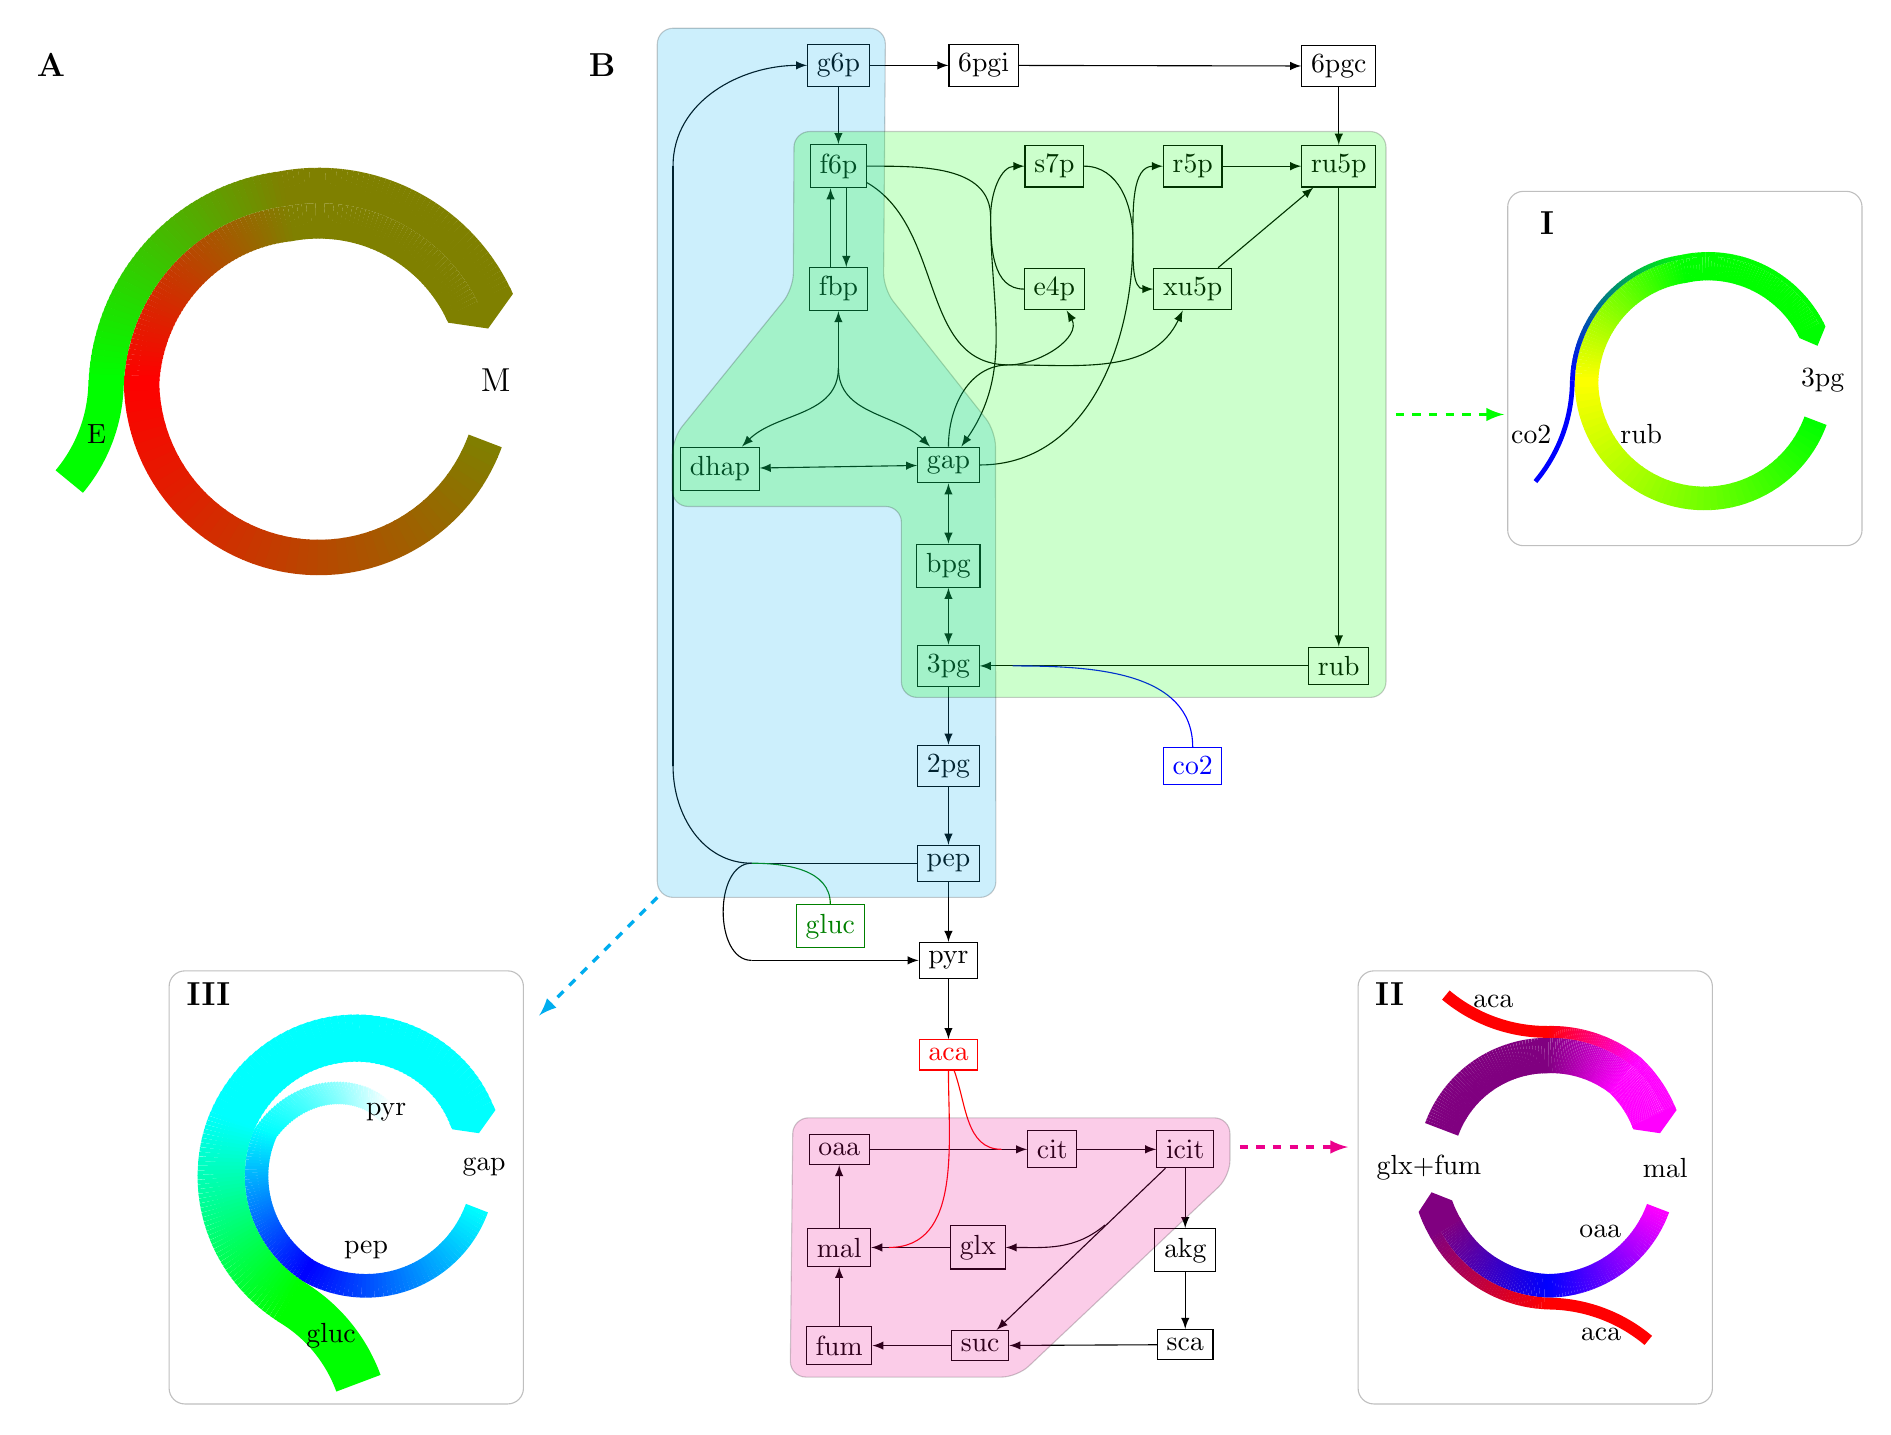
\begin{tikzpicture}
  \node[rectangle,draw] (g6p) {g6p};
  \node[rectangle,draw,below=of g6p.center] (f6p) {f6p};
  \node[rectangle,draw,below=of f6p] (fbp) {fbp};
  \node[rectangle,draw,shape=coordinate,below=of fbp.center](fbamid) {};
  \node[rectangle,draw,below left=of fbamid.center] (dhap) {dhap};
  \node[rectangle,draw,below right=of fbamid] (gap) {gap};
  \node[rectangle,draw,below=of gap.center] (bpg) {bpg};
  \node[rectangle,draw,below=of bpg.center] (3pg) {3pg};
  \node[rectangle,draw,below=of 3pg.center] (2pg) {2pg};
  \node[rectangle,draw,below=of 2pg.center] (pep) {pep};
  \node[rectangle,draw,below=of pep.center] (pyr) {pyr};
  \node[rectangle,draw,below=of pyr.center,glyext] (aca) {aca};
  \node[shape=coordinate,below=of aca] (dummyglta) {};
  \node[rectangle,draw,left=of dummyglta] (oaa) {oaa};
  \node[rectangle,draw,right=of dummyglta] (cit) {cit};
  \node[rectangle,draw,right=of cit] (icit) {icit};
  \node[rectangle,draw,below=of icit.center] (akg) {akg};
  \node[rectangle,draw,below=of akg.center] (sca) {sca};
  \node[rectangle,draw,below=of oaa.center] (mal) {mal};
  \node[rectangle,draw,below=of mal.center] (fum) {fum};
  \node[rectangle,draw,right=of mal] (glx) {glx};
  \node[rectangle,draw,right=of fum] (suc) {suc};
  \node[rectangle,draw,right=of g6p] (6pgi) {6pgi};
  \node[rectangle,draw,shape=coordinate,right=of f6p] (s7pspace) {};
  \node[rectangle,draw,right=of s7pspace] (s7p) {s7p};
  \node[rectangle,draw,right=of s7p] (r5p) {r5p};
  \node[rectangle,draw,right=of r5p] (ru5p) {ru5p};
  \node[rectangle,draw,above=of ru5p.center] (6pgc) {6pgc};
  \node[rectangle,draw,] at (fbp.center -| s7p.center) (e4p) {e4p};
  \node[rectangle,draw,] at(e4p.center -| r5p.center) (xu5p) {xu5p};
  \node[rectangle,draw,] at(3pg.center -| ru5p.center) (rub) {rub};
  \node[rectangle,draw,cbbext] at(2pg -| xu5p.center) (co2) {co2};
  \draw[->] (g6p) -- (f6p);
  \draw[->] ([xshift=0.1cm]f6p.south) -- ([xshift=0.1cm]fbp.north);
  \draw[<-] ([xshift=-0.1cm]f6p.south) -- ([xshift=-0.1cm]fbp.north);
  \draw [<-] (fbp) [out=-90,in=90] to (fbamid);
  \draw [->] (fbamid) [out=-90,in=45] to (dhap);
  \draw [->] (fbamid) [out=-90,in=135] to (gap);
  \draw [<->] (dhap) -- (gap);
  \draw[<->] (gap) -- (bpg);
  \draw[<->] (bpg) -- (3pg);
  \draw[->] (3pg) -- (2pg);
  \draw[->] (2pg) -- (pep);
  \draw[->] (pep) -- (pyr);
  \draw[->] (pyr) -- (aca);
  \draw[->] (oaa) -- (cit) node [pos=0.9] (midglta) {};
  \draw [glyext] (aca) [out=-70,in=180] to (midglta);
  \draw[->] (cit) -- (icit);
  \draw[->] (icit) -- (suc) node [pos=0.3] (midacea) {};
  \draw[->] (midacea) [out=220,in=0] to (glx);
  \draw[->] (icit) -- (akg);
  \draw[->] (akg) -- (sca);
  \draw[->] (sca) -- (suc);
  \draw[->] (suc) -- (fum);
  \draw[->] (fum) -- (mal);
  \draw[->] (glx) -- (mal) node [pos=0.9] (midaceb) {};
  \draw[->] (mal) -- (oaa);
  \draw[glyext] (aca) [out=-90,in=0] to (midaceb);
  \draw[->] (g6p) -- (6pgi);
  \draw[->] (6pgi) -- (6pgc);
  \draw[->] (6pgc) -- (ru5p);
  \draw[<-] (ru5p) -- (xu5p);
  \draw[<-] (ru5p) -- (r5p);
  \path[] (r5p) -- (gap) coordinate [pos=0.2] (midtkt1) {};
  \draw[<-] (xu5p) [out=180,in=-90] to (midtkt1);
  \draw[] (midtkt1) [out=90,in=0] to (s7p);
  \draw[<-] (r5p) [out=180,in=90] to (midtkt1);
  \draw[] (midtkt1) [out=270,in=0] to (gap);
  \path[] (e4p) -- (gap) coordinate [pos=0.4] (midtkt2) {};
  \draw[<-] (e4p) [out=-60,in=0] to (midtkt2);
  \draw[] (midtkt2) [out=180,in=90] to (gap);
  \draw[<-] (xu5p) [out=245,in=0] to (midtkt2);
  \draw[] (midtkt2) [out=180,in=-30] to (f6p);
  \path[] (e4p) -- (s7pspace) coordinate [pos=0.5] (midtal) {};
  \draw[] (midtal) [out=90,in=0] to (f6p);
  \draw[<-] (s7p) [out=180,in=90] to (midtal);
  \draw[] (midtal) [out=-90,in=180] to (e4p);
  \draw[<-] (gap) [out=55,in=-90] to (midtal);
  \node[rectangle,draw,shape=coordinate,left=of dhap.center] (pts2) {};
  \node[rectangle,draw,gluccol,shift={(-1.5,-0.8)}] at (pep.center) (gluc) {gluc};
  \node[rectangle,draw,shape=coordinate,left=2.5cm of pep.center] (pts3) {};
  \draw[] (pep) [out=180,in=0] to (pts3);
  \draw[gluccol] (gluc) [out=90,in=0] to (pts3);
  \node[rectangle,draw,shape=coordinate,left=2.5cm of pyr.center] (pts5) {};
  \draw[] (pts3) [out=180,in=180] to (pts5);
  \draw[->] (pts5) [out=0,in=180] to (pyr);
  \node[rectangle,draw,shape=coordinate,left=2.1cm of f6p.center] (ptstop) {};
  \node[rectangle,draw,shape=coordinate] at(ptstop |- 2pg.center) (ptsbottom) {};
  \draw[] (pts3) [in=-90,out=180] to (ptsbottom);
  \draw[] (ptsbottom) [in=-90,out=90] to (ptstop);
  \draw[->] (ptstop) [in=180,out=90] to (g6p);
  \draw[->] (ru5p) [out=-90,in=90] to (rub);
  \draw[->] (rub) -- (3pg) coordinate [pos=0.9] (rubisco); 
  \draw[cbbext] (co2) [out=90,in=0] to (rubisco);
  \node[shape=coordinate,shift={(-\highlightrad,-\highlightrad)}] at (pep.south -| ptsbottom) (ptsbottomlimit) {};
  \node[shape=coordinate,shift={(-\highlightrad,\highlightrad)}] at (g6p.north -| ptstop) (ptstoplimit) {};

  \draw[opacity=0.2,fill=ptsinit,rounded corners=\highlightrad] ([shift={(\highlightrad,\highlightrad)}]g6p.north east) -- ([xshift=\highlightrad] fbp.east) -- ([shift={(\highlightrad,\highlightrad)}]gap.north east)--([shift={(\highlightrad,-\highlightrad)}]pep.south east) -- (ptsbottomlimit) -- (ptstoplimit) -- cycle;

  \draw[very thick,dashed,cyan,->] (ptsbottomlimit) -- ++(-1.5cm,-1.5cm); 

  \draw[opacity=0.2,fill=glyinit,rounded corners=\highlightrad] ([shift={(-\highlightrad,2*\highlightrad)}]oaa.west) -- ([shift={(\highlightrad,2*\highlightrad)}]icit.east) -- node[midway] (glyshadedmid) {}([shift={(\highlightrad,-0.5*\highlightrad)}]icit.south east) -- ([shift={(0.5*\highlightrad,-2*\highlightrad)}]suc.east) -- ([shift={(-\highlightrad,-2*\highlightrad)}]fum.west) -- cycle;

  \draw[very thick,dashed,magenta,->] (glyshadedmid) -- ++(1.5cm,0cm); 

  \node[shape=coordinate] at (dhap.south -| gap.west) (cbbmid) {};
  \draw[opacity=0.2,fill=cbbinit,rounded corners=\highlightrad] ([shift={(-\highlightrad,2.2*\highlightrad)}]f6p.west) -- ([shift={(3*\highlightrad,2.2*\highlightrad)}]ru5p.center) -- node[midway] (cbbshadedmid) {} ([shift={(3*\highlightrad,-2*\highlightrad)}]rub.center) -- ([shift={(-\highlightrad,-2*\highlightrad)}]3pg.west) -- ([shift={(-\highlightrad,-\highlightrad)}]cbbmid) -- ([shift={(-0.5*\highlightrad,-\highlightrad)}]dhap.south west) -- ([shift={(-0.5*\highlightrad,0.5*\highlightrad)}]dhap.north west) -- ([xshift=-\highlightrad]fbp.west) -- cycle;

  \draw[very thick,dashed,green,->] (cbbshadedmid) -- ++(1.5cm,0cm); 

    \newlength\imrad;
    \newlength\ierad;
    \newlength\esrad;
    \newlength\emrad;
    \newlength\eerad;
    \pgfmathsetlength{\imrad}{\autocatalrad-\blendfrac*\arcwidth};
    \pgfmathsetlength{\ierad}{\autocatalrad-0.5*\arcwidth};
    \pgfmathsetlength{\esrad}{\autocatalrad+\arcwidth};
    \pgfmathsetlength{\emrad}{\autocatalrad+\arcwidth-\blendfrac*\arcwidth};
    \pgfmathsetlength{\eerad}{\autocatalrad+0.5*\arcwidth};

  %% CBB cycle
  \begin{scope} [shift={(11cm,-4cm)},radius=2cm]
    \newlength\cbbimrad;
    \newlength\cbbierad;
    \newlength\cbbesrad;
    \newlength\cbbemrad;
    \newlength\cbbeerad;
    \newlength\cbbwidth;
    \newlength\cbbtotwidth;
    \pgfmathsetlength{\cbbwidth}{\arcwidth*0.2};
    \pgfmathsetlength{\cbbtotwidth}{\cbbwidth+\arcwidth};
    \pgfmathsetlength{\cbbimrad}{\autocatalrad-\blendfrac*0.5*\cbbtotwidth};
    \pgfmathsetlength{\cbbierad}{\autocatalrad-0.5*\cbbwidth};
    \pgfmathsetlength{\cbbesrad}{\autocatalrad+0.5*\cbbtotwidth};
    \pgfmathsetlength{\cbbemrad}{\autocatalrad+0.5*\cbbtotwidth-\blendfrac*0.5*\cbbtotwidth};
    \pgfmathsetlength{\cbbeerad}{\autocatalrad+0.5*\arcwidth};

    \shadedarc{-20}{-180}{\autocatalrad}{\autocatalrad}{cbbmed}{cbbinit};
    \shadedarc{100}{180}{\cbbimrad}{\autocatalrad}{cbbmed}{cbbinit};
    \coloredarc{25}{100}{\cbbierad}{\cbbimrad}{cbbmed!0.5!cbbinit};
    \shadedarc[\cbbwidth]{100}{180}{\cbbemrad}{\cbbesrad}{cbbext}{cbbinit};
    \coloredarc[\cbbwidth]{25}{100}{\cbbeerad}{\cbbemrad}{cbbext!0.5!cbbinit};

%% \assimilatedcol input arc
        \draw[color=cbbext!99.5!cbbinit,line width=\cbbwidth]
        (\fromang:\autocatalrad+0.5*\arcwidth+0.5*\cbbwidth)
        arc (0:\inputang:2cm)
        node [pos=0.5,color=black,anchor=east] (co2c) {co2};
%% arrowhead
    \fill[cbbext!0.5!cbbinit]
      (\fromang+\deltaang+1:\autocatalrad-0.5*\arcwidth-0.5*\cbbwidth)
      arc (\fromang+\deltaang+1:\fromang+\deltaang-1:\autocatalrad-0.5*\arcwidth-0.5*\cbbwidth)
      -- (\fromang+\deltaang-1-\protrude:\autocatalrad)
      -- (\fromang+\deltaang-1:\autocatalrad+0.5*\arcwidth+0.5*\cbbwidth)
      arc (\fromang+\deltaang-1:\fromang+\deltaang+1:\autocatalrad+0.5*\arcwidth+0.5*\cbbwidth)
      -- cycle;

%% metabolites
        \node at (0:\autocatalrad) (3pgc) {3pg};
        \node at (220:\autocatalrad-4.5mm) (rubc) {rub};

  \end{scope}
%%%%%%%%%%%%%%%%%%%%%
%Todo:
% add dashed lines from highlighted cycles in central metabolism to specific cycles
% add generic autocatalytic cycle as panel A at top left
% send to ron
%%%%%%%%%%%%%%%%%%%%


  %glyoxilate cycle
\begin{scope} [shift={(9cm,-14cm)},radius=2cm]
    \newlength\glyimrad;
    \newlength\glyierad;
    \newlength\glyesrad;
    \newlength\glyemrad;
    \newlength\glyeerad;
    \newlength\glywidth;
    \newlength\glytotwidth;
    \newlength\glyfinwidth;
    \newlength\glyimmrad;
    \newlength\glyemmrad;
    \newlength\glyemmmrad;
    \newlength\glyeamrad;
    \pgfmathsetlength{\glywidth}{\arcwidth*0.5};
    \pgfmathsetlength{\glytotwidth}{\glywidth+\arcwidth};
    \pgfmathsetlength{\glyfinwidth}{\glytotwidth+\glywidth};
    \pgfmathsetlength{\glyimrad}{\autocatalrad-\blendfrac*0.5*\glywidth};
    \pgfmathsetlength{\glyimmrad}{\autocatalrad-0.5*\glywidth};
    \pgfmathsetlength{\glyemmrad}{\glyimmrad+0.5*\glytotwidth};
    \pgfmathsetlength{\glyemmmrad}{\glyemmrad+0.5*\glywidth};
    \pgfmathsetlength{\glyeamrad}{\autocatalrad+0.5*\glytotwidth};
    \pgfmathsetlength{\glyierad}{\autocatalrad-0.5*\glywidth};
    \pgfmathsetlength{\glyesrad}{\autocatalrad+0.5*\glytotwidth};
    \pgfmathsetlength{\glyemrad}{\autocatalrad+0.5*\glyfinwidth-\blendfrac*0.5*\glywidth};
    \pgfmathsetlength{\glyeerad}{\autocatalrad+0.5*\glytotwidth};

    \shadedarc{-20}{-90}{\autocatalrad}{\autocatalrad}{glymed}{glyinit};
    \shadedarc{-150}{-90}{\glyimmrad}{\autocatalrad}{glymed}{glyinter};
    \shadedarc[\glywidth]{-150}{-90}{\glyemmrad}{\glyeamrad}{glyext}{glyinter};

    \draw[color=glyext!99.5!glyinit,line width=\glywidth] (-90:\autocatalrad+0.5*\glytotwidth) arc(90:50:2cm) node [pos=0.5,color=black,anchor=north] (acac) {aca};

    \coloredarc[\glytotwidth]{160}{90}{\glyimmrad}{\glyimmrad}{glyinter};

    \draw[color=glyext!99.5!glyinit,line width=\glywidth] (90:\glyemmmrad) arc(-90:-130:2cm) node [pos=0.5,color=black,anchor=south] (acac) {aca};

    \shadedarc[\glytotwidth]{50}{90}{\glyimrad}{\glyimmrad}{glyinter}{glyinit};
    \coloredarc[\glytotwidth]{50}{25}{\glyimrad}{\glyierad}{glyext!0.5!glyinit};

    \shadedarc[\glywidth]{90}{50}{\glyemmmrad}{\glyemrad}{glyext!0.5!glyinit}{glyext};
    \coloredarc[\glywidth]{50}{25}{\glyemrad}{\glyeerad}{glyext!0.5!glyinit};


    \node at (0:\autocatalrad) (malc) {mal};
    \node at (180:\autocatalrad) (glxc) {glx+fum};
    \node at (-50:\autocatalrad-4.5mm) (oaa) {oaa};

  \fill[glyext!0.5!glyinit] (\fromang+\deltaang+1:\autocatalrad-\arcwidth) arc (\fromang+\deltaang+1:\fromang+\deltaang-1:\autocatalrad-\arcwidth)
       -- (\fromang+\deltaang-1-\protrude:\autocatalrad) -- (\fromang+\deltaang-1:\autocatalrad+\arcwidth) arc (\fromang+\deltaang-1:\fromang+\deltaang+1:\autocatalrad+\arcwidth)
       -- cycle;

  \fill[glyinter] (-149:\autocatalrad-\arcwidth+0.5*\glywidth) arc (-149:-161:\autocatalrad-\arcwidth+0.5*\glywidth)
       -- (-161-\protrude:\autocatalrad) -- (-161:\autocatalrad+\arcwidth-0.5*\glywidth) arc (-161:-149:\autocatalrad+\arcwidth-0.5*\glywidth)
       -- cycle;
  \end{scope}


  %pts cycle
 \begin{scope} [shift={(-6cm,-14cm)},radius=2cm]
    \newlength\ptsierad;
    \newlength\ptsimrad;
    \newlength\ptsarcwidth;
    \newlength\ptsesrad;
    \newlength\ptsemrad;
    \pgfmathsetlength{\ptsierad}{\autocatalrad*0.5};
    \pgfmathsetlength{\ptsimrad}{\autocatalrad-0.5*\arcwidth};
    \pgfmathsetlength{\ptsarcwidth}{2*\arcwidth};
    \pgfmathsetlength{\ptsesrad}{\autocatalrad+0.5*\arcwidth+0.5*\ptsarcwidth};
    \pgfmathsetlength{\ptsemrad}{\autocatalrad+0.5*\ptsarcwidth};

    \shadedarc{-20}{-120}{\autocatalrad}{\autocatalrad}{ptsmed}{ptsinit};
    \shadedarc{160}{240}{\ptsimrad}{\autocatalrad}{ptsmed}{ptsinit};
    \shadedarc{70}{160}{\ptsierad}{\ptsimrad}{ptsext!0.5!ptsinit}{white};
    \shadedarc[\ptsarcwidth]{160}{240}{\ptsemrad}{\ptsesrad}{ptsext}{ptsinit};
    \coloredarc[\ptsarcwidth]{25}{160}{\autocatalrad}{\ptsemrad}{ptsext!0.5!ptsinit};

  \fill[ptsext!0.5!ptsinit] (\fromang+\deltaang+1:\autocatalrad-\arcwidth) arc (\fromang+\deltaang+1:\fromang+\deltaang-1:\autocatalrad-\arcwidth)
       -- (\fromang+\deltaang-1-\protrude:\autocatalrad) -- (\fromang+\deltaang-1:\autocatalrad+\arcwidth) arc (\fromang+\deltaang-1:\fromang+\deltaang+1:\autocatalrad+\arcwidth)
       -- cycle;

       %% \assimilatedcol input arc
       \draw[color=ptsext!99.5!ptsinit,line width=\ptsarcwidth] (240:\ptsesrad) arc(60:20:2cm) node [pos=0.5,color=black] (glucc) {gluc};
    \node at (0:\autocatalrad) (gapc) {gap};
    \node at (270:\autocatalrad-4.5mm) (pepc) {pep};
    \node at (70:\ptsierad) (pyrc) {pyr};
  \end{scope}

  %generic cycle
\begin{scope} [shift={(-6.6cm,-4cm)}]
    \shadedarc[\autocatalscale*\arcwidth]{-20}{-180}{\autocatalscale*\autocatalrad}{\autocatalscale*\autocatalrad}{genmed}{geninit};
    \shadedarc[\autocatalscale*\arcwidth]{100}{180}{\autocatalscale*\imrad}{\autocatalscale*\autocatalrad}{genmed}{geninit};
    \shadedarc[\autocatalscale*\arcwidth]{100}{180}{\autocatalscale*\emrad}{\autocatalscale*\esrad}{genext}{geninit};
    \coloredarc[\autocatalscale*\arcwidth]{25}{100}{\autocatalscale*\eerad}{\autocatalscale*\emrad}{genext!0.5!geninit};
    \coloredarc[\autocatalscale*\arcwidth]{25}{100}{\autocatalscale*\ierad}{\autocatalscale*\imrad}{genext!0.5!geninit};

  \fill[genext!0.5!geninit] (\fromang+\deltaang+1:\autocatalscale*\autocatalrad-\autocatalscale*\arcwidth) arc (\fromang+\deltaang+1:\fromang+\deltaang-1:\autocatalscale*\autocatalrad-\autocatalscale*\arcwidth)
       -- (\fromang+\deltaang-1-\protrude:\autocatalscale*\autocatalrad) -- (\fromang+\deltaang-1:\autocatalscale*\autocatalrad+\autocatalscale*\arcwidth) arc (\fromang+\deltaang-1:\fromang+\deltaang+1:\autocatalscale*\autocatalrad+\autocatalscale*\arcwidth)
       -- cycle;

       %% \assimilatedcol input arc
       \draw[color=genext!99.5!geninit,line width=\autocatalscale*\arcwidth] (180:\autocatalscale*\esrad) arc(0:-40:2cm) node [pos=0.5,color=black] (ext) {E};
    \node at (0:\autocatalscale*\autocatalrad) (int) {\large M};
  \end{scope}
  %\draw[lightgray,rounded corners=\highlightrad] (-10.3,-8) rectangle +(6.8,8.5);
  \node at (-10cm,0) (A) {\large \textbf A};
  \node at (-3cm,0) (B) {\large  \textbf B};
  \draw[lightgray,rounded corners=\highlightrad] (8.5,-6.1) rectangle +(4.5,4.5);
  \node at (9cm,-2cm) (I) {\large  \textbf{I}};
  \draw[lightgray,rounded corners=\highlightrad] (6.6,-17) rectangle +(4.5,5.5);
  \node at (7cm,-11.8cm) (II) {\large  \textbf {II}};
  \draw[lightgray,rounded corners=\highlightrad] (-8.5,-17) rectangle +(4.5,5.5);
  \node at (-8cm,-11.8cm) (III) {\large  \textbf {III}};

\end{tikzpicture}
}
\caption{
(A) A basic autocatalytic cycle uses the internal metabolite, M, in order to assimilate an external metabolite, E, into the cycle, increasing the amount of M.
(B) Three representative autocatalytic cycles in central carbon metabolism: (I) The Calvin Benson Bassham cycle; (II) The glyoxilate cycle; (III) A cycle using the PTS system to assimilate glucose.
}
\end{figure}
\end{document}
